\documentclass[10pt]{beamer}
\usetheme{Madrid}
\usepackage[utf8]{inputenc}
\usepackage[french]{babel}
\usepackage[T1]{fontenc}
\usepackage{amsmath}
\usepackage{amsfonts}
\usepackage{amssymb}
\usepackage{graphicx}
\usepackage{relsize}
\usepackage{subcaption}
\usepackage{amsmath}
\usepackage{listings}
\usepackage{xcolor}
\usepackage{multicol}

\author{TRAN-THUONG Tien-Thinh}
\date{2021-2022}
% \title{Reconnaissance vocale lors d’appel d’urgence grâce à un réseau de neurones}
\title{Présentation}
\graphicspath{{Affiche/0-ReconnaissanceVocale/}{Affiche/1-Introduction/}{Affiche/2-Activation-Gradient/}{Affiche/4-XOR/}}
\lstset{inputpath={Affiche/99-Code/}}
\newcommand{\norme}[1]{\| #1 \|}

\definecolor{codegreen}{rgb}{0,0.6,0}
\definecolor{codegray}{rgb}{0.5,0.5,0.5}
\definecolor{codepurple}{rgb}{0.58,0,0.82}
\definecolor{backcolour}{rgb}{0.95,0.95,0.92}
\lstdefinestyle{mystyle}{
    backgroundcolor=\color{backcolour},   
    commentstyle=\color{codegreen},
    keywordstyle=\color{magenta},
    numberstyle=\tiny\color{codegray},
    stringstyle=\color{codepurple},
    basicstyle=\ttfamily\footnotesize,
    breakatwhitespace=false,         
    breaklines=true,                 
    captionpos=b,                    
    keepspaces=true,                 
    numbers=left,                    
    numbersep=5pt,                  
    showspaces=false,                
    showstringspaces=false,
    showtabs=false,                  
    tabsize=2
}
\lstset{style=mystyle}

\begin{document}

\begin{frame}
\titlepage
\end{frame}

\begin{frame}{Problématique}
\begin{alert}{D'après le ministère de la Santé : }
Il y a eu plus de \textbf{31 millions} d'appels d'urgence en 2018. Seuls \textbf{69\%} des appels étaient décrochés dans la minute.
\end{alert}
\begin{block}{Objectif}
Utiliser la reconnaissance vocale par réseau de neurones pour aider à classifier rapidement l'objet d'un appel.
\end{block}
\end{frame}


\begin{frame}{La reconnaissance automatique de la parole}
\begin{itemize}
	\item[1] Le traitement acoustique 
	\item[2] L'apprentissage automatique
	\item[3] Le décodage
\end{itemize}
\begin{figure}
	\begin{subfigure}[]{0.3\textwidth}
		\centering
		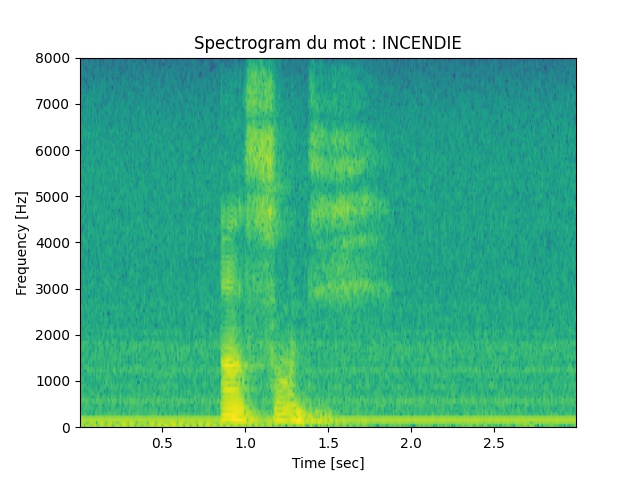
\includegraphics[height=50px]{1-Incendie-3.jpg}
  		\caption{Spectrogramme}
	\end{subfigure}
	\begin{subfigure}[]{0.3\textwidth}
		\centering
		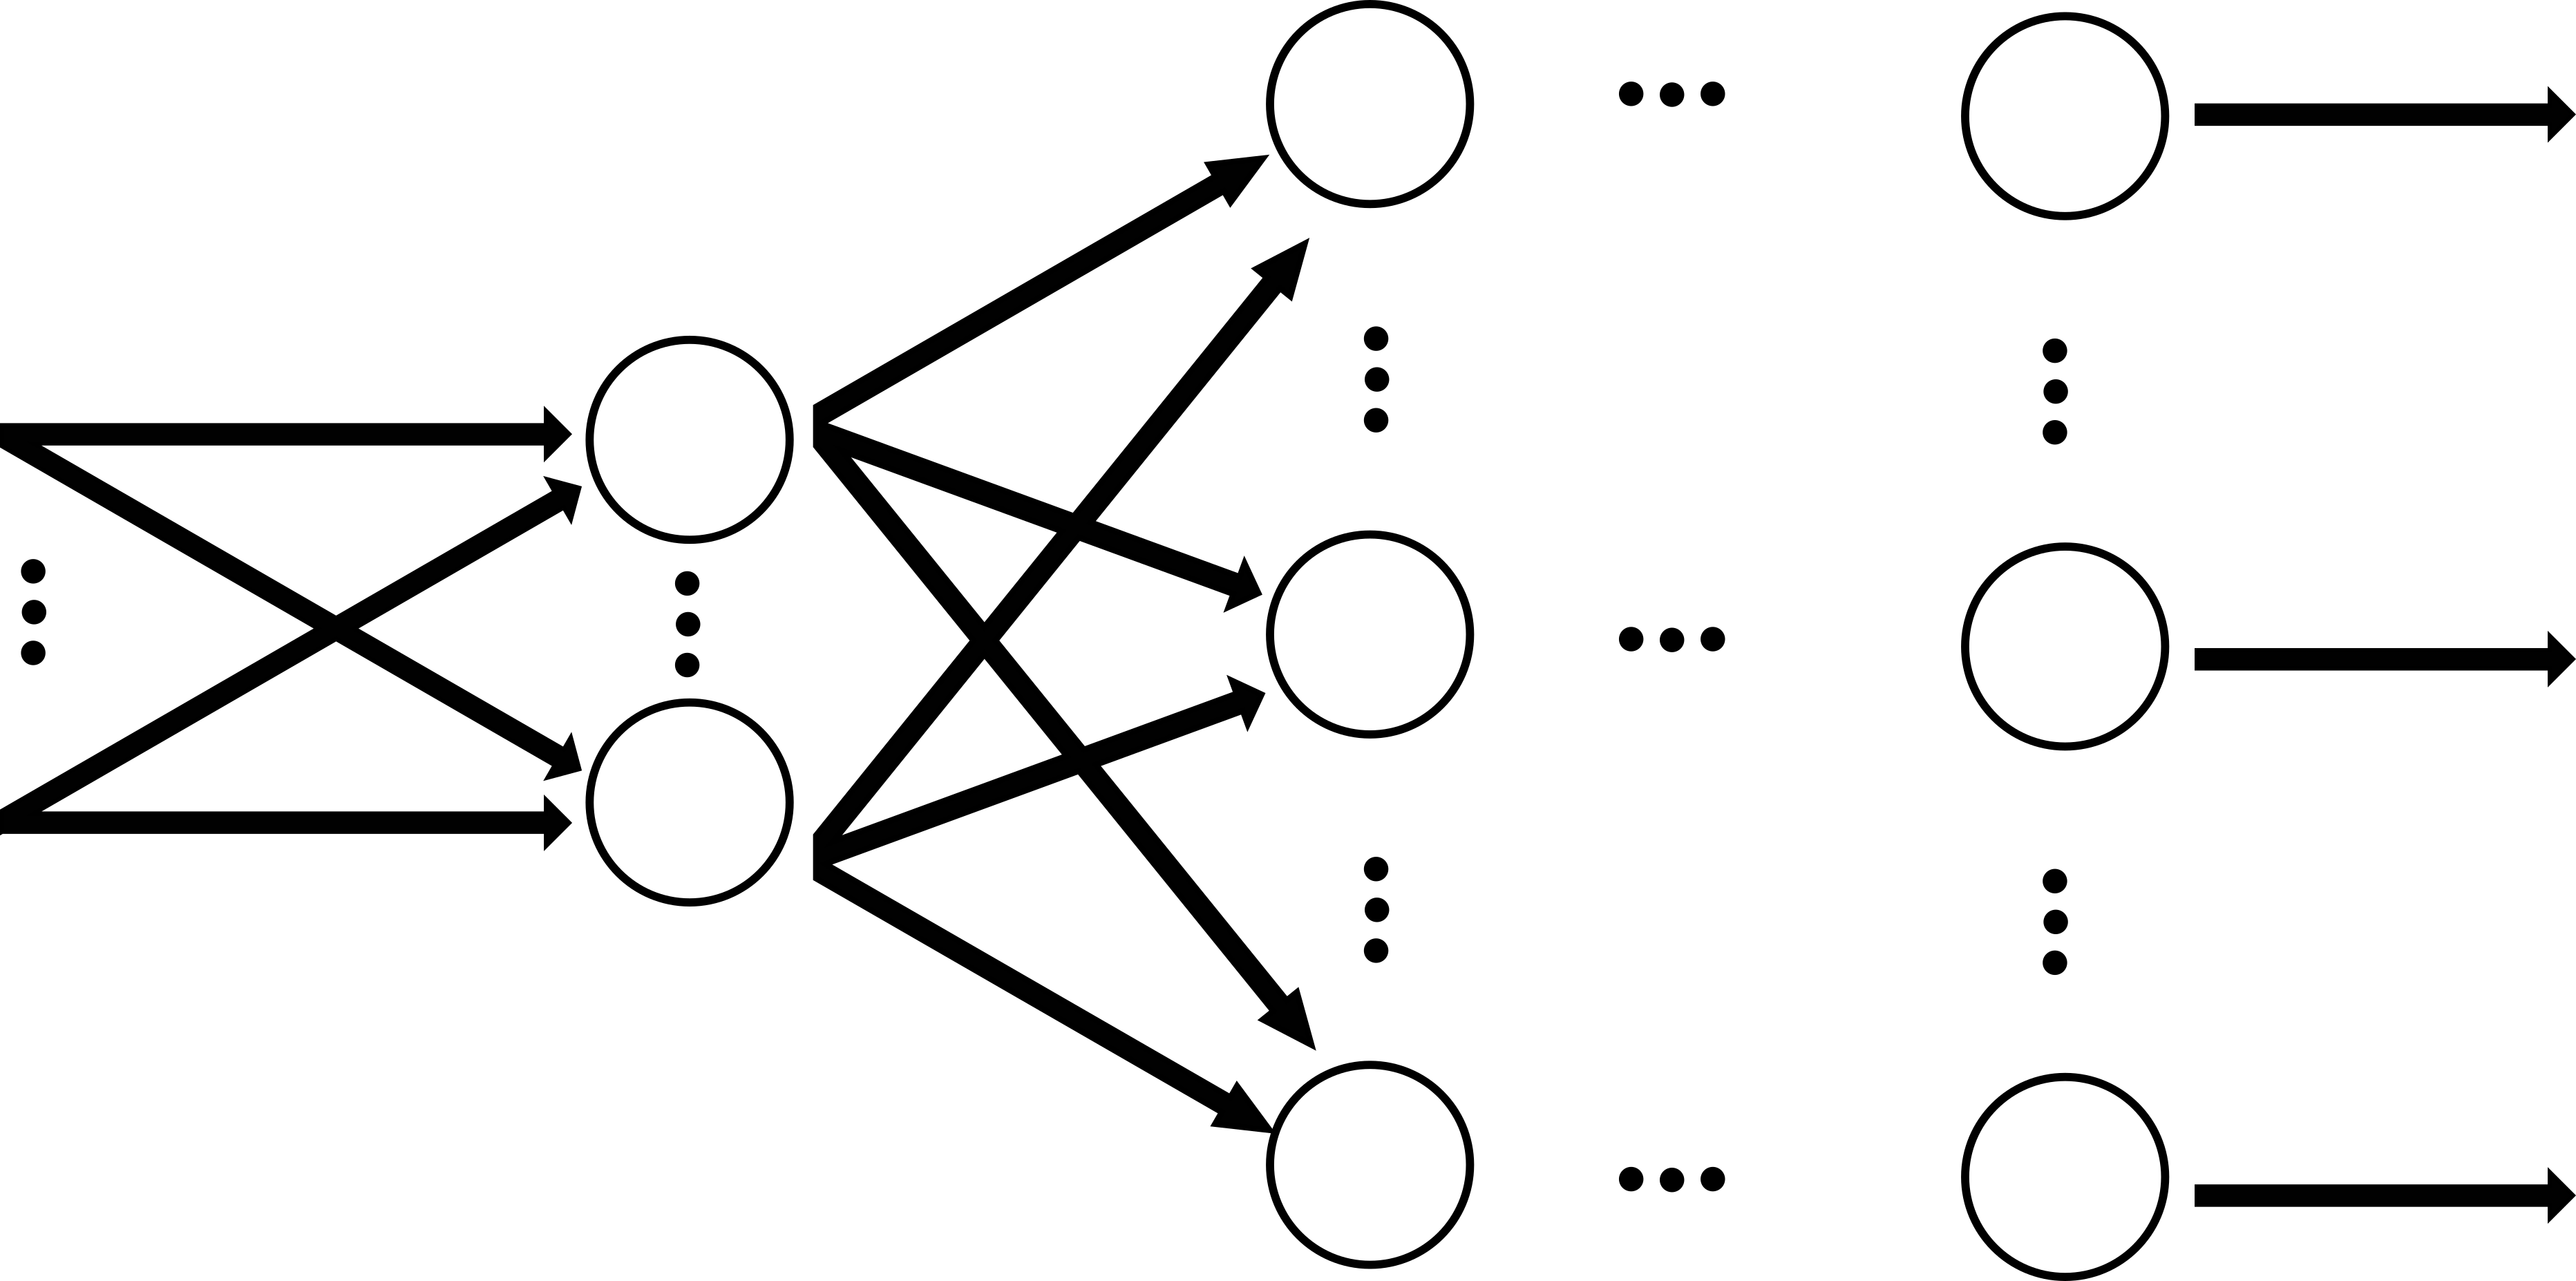
\includegraphics[height=50px]{2-Reseau.png}
  		\caption{Réseau de neurones}
	\end{subfigure}
	\begin{subfigure}[]{0.3\textwidth}
		\centering
		
\includegraphics[height=50px]{3-Matching.png}
		\caption{Correspondance phonétique}
	\end{subfigure}
\end{figure}
\end{frame}

% 1-INTRODUCTION
\section{I - Introduction}
\begin{frame}{I - Introduction}
\begin{block}{Présentation du modèle du Perceptron}
McCulloh et Pitts introduise le modèle du Perceptron en 1943, basé sur le fonctionnement du neurone humain.
\end{block}
\end{frame}

\begin{frame}{I - Introduction}
\begin{figure}
	\centering
    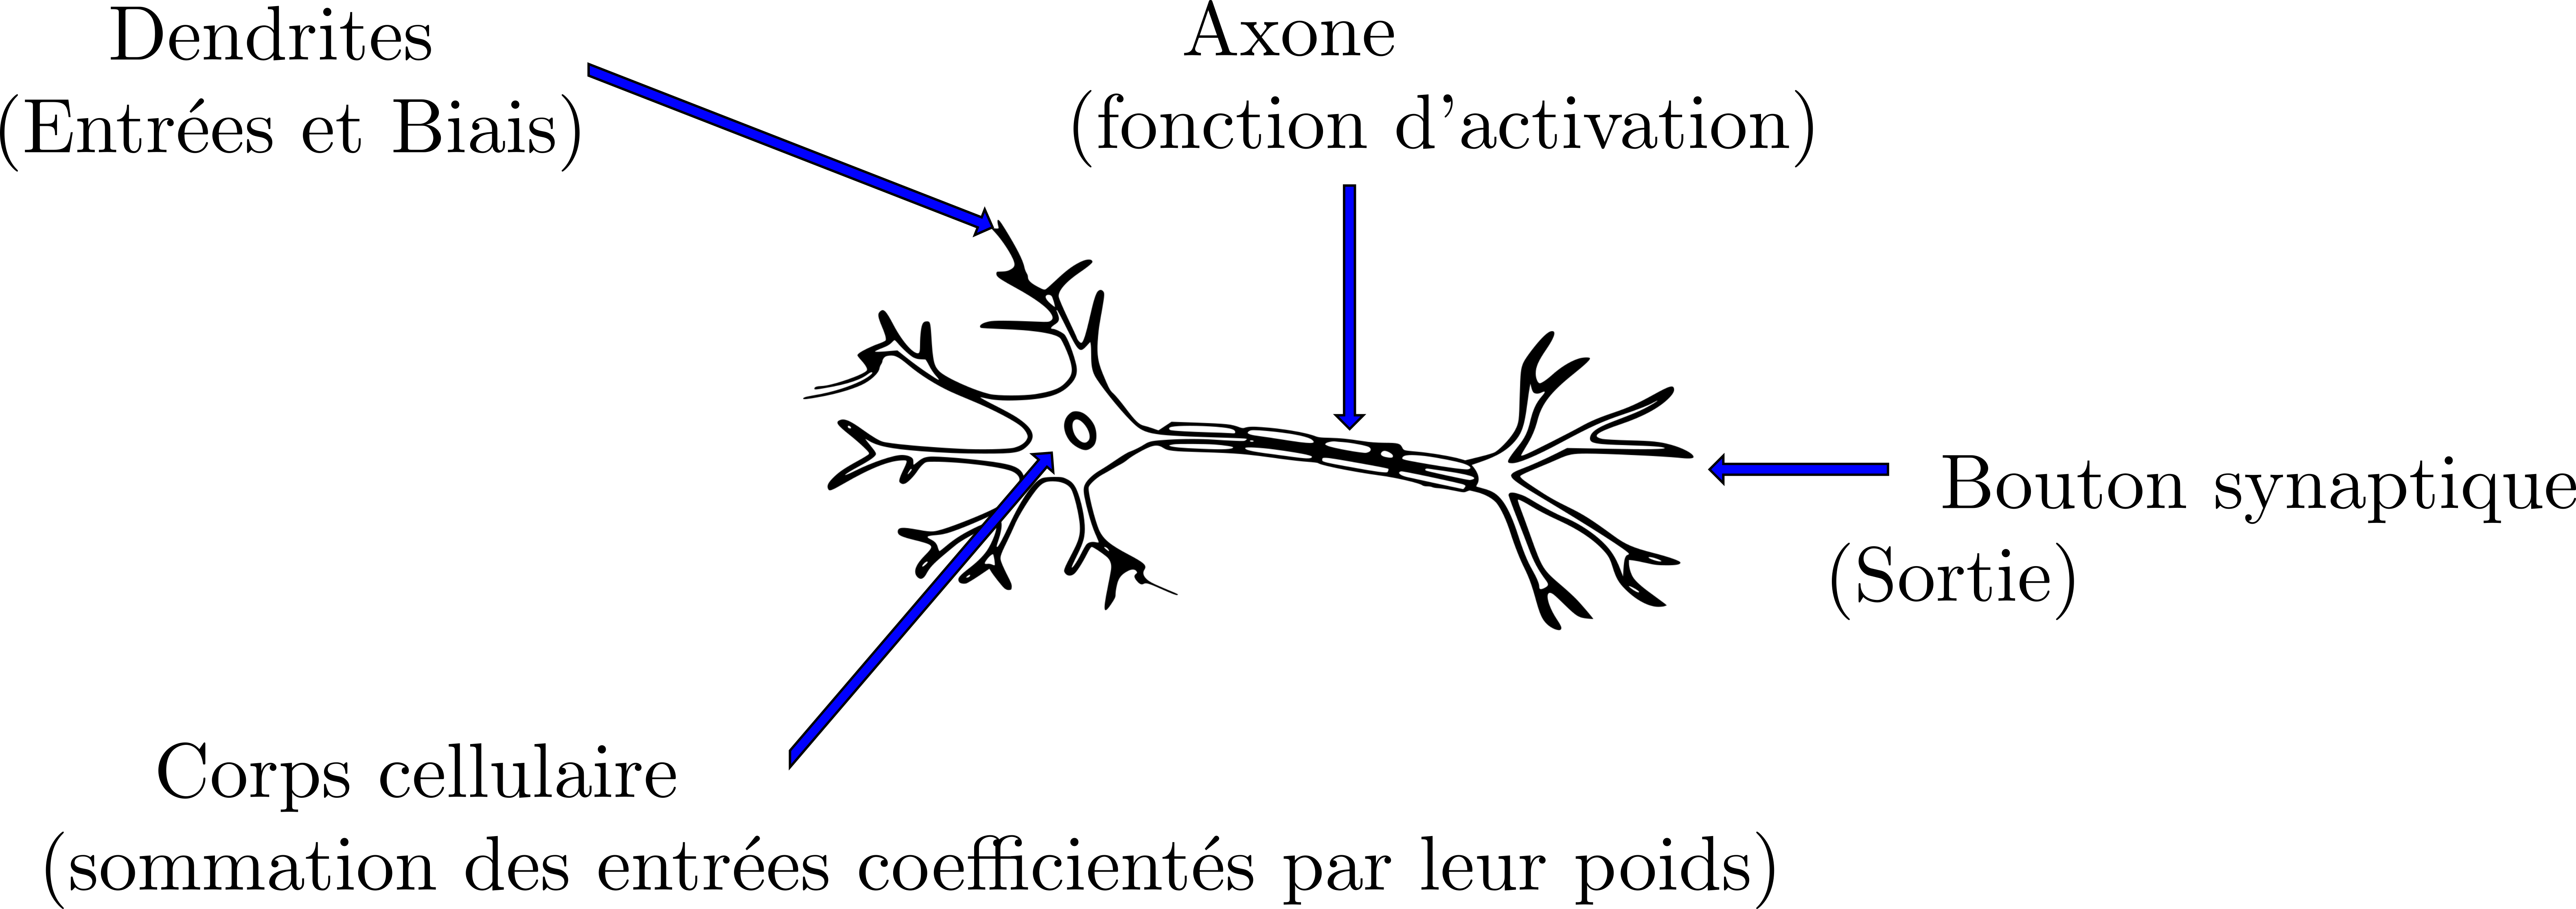
\includegraphics[height=75px]{2-Neurone.png}
	\caption{Schéma d'un neurone}	
\end{figure}
\begin{figure}
	\centering
    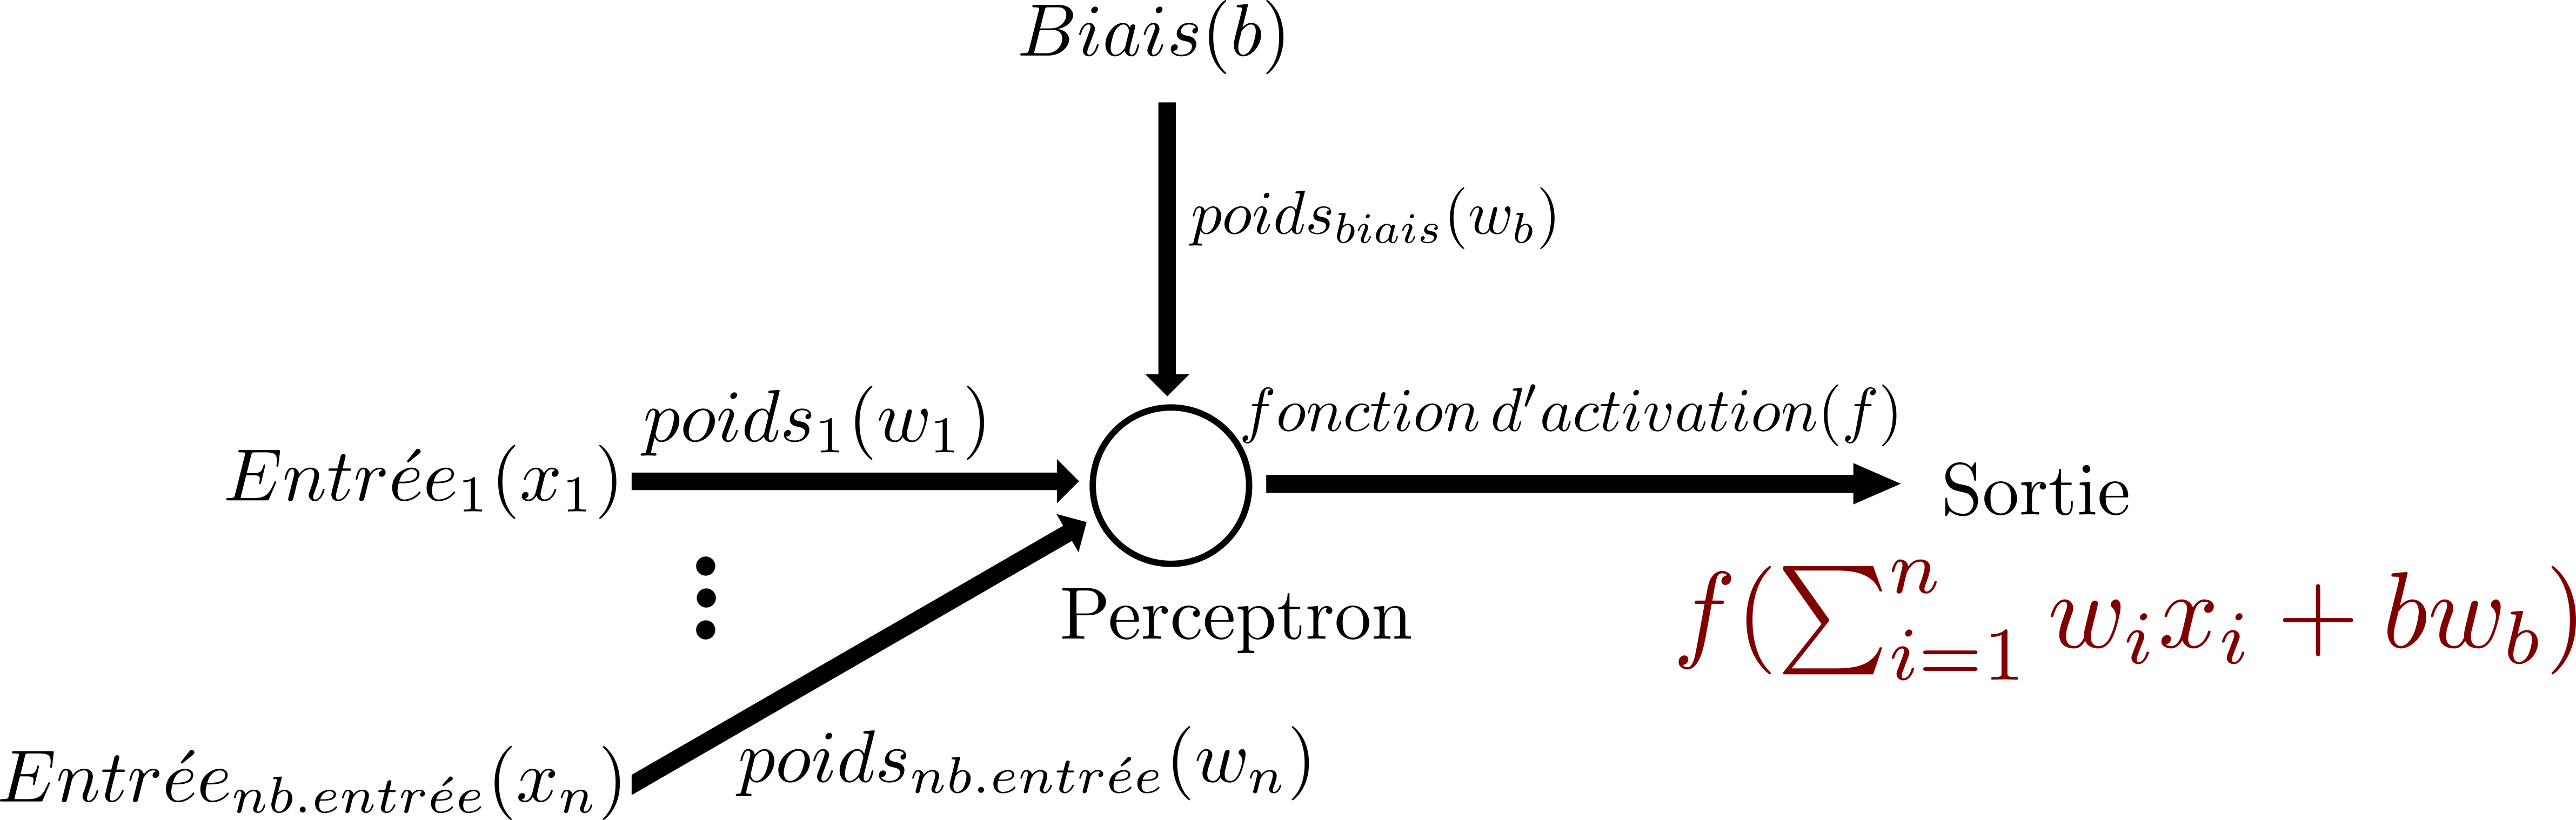
\includegraphics[height=75px]{1-Perceptron.png}
	\caption{Schéma d'un perceptron}	
\end{figure}
\end{frame}

% 2-Fonction d'activation
\section{II - Fonction d'activation}
\begin{frame}{II - Fonction d'activation}
\begin{block}{Fonction d'activation}
Sans l'utilisation de la fonction d'activation, le neurone est multilinéaire par rapport à ses entrées, il n'est donc capable que de faire des régressions linéaires sur les données d'entrées. \\
Les fonctions d'activation permettent donc une classification non linéaire.
\end{block}
\end{frame}


\begin{frame}{II - Représentation informatique}
\begin{figure}
	\centering
    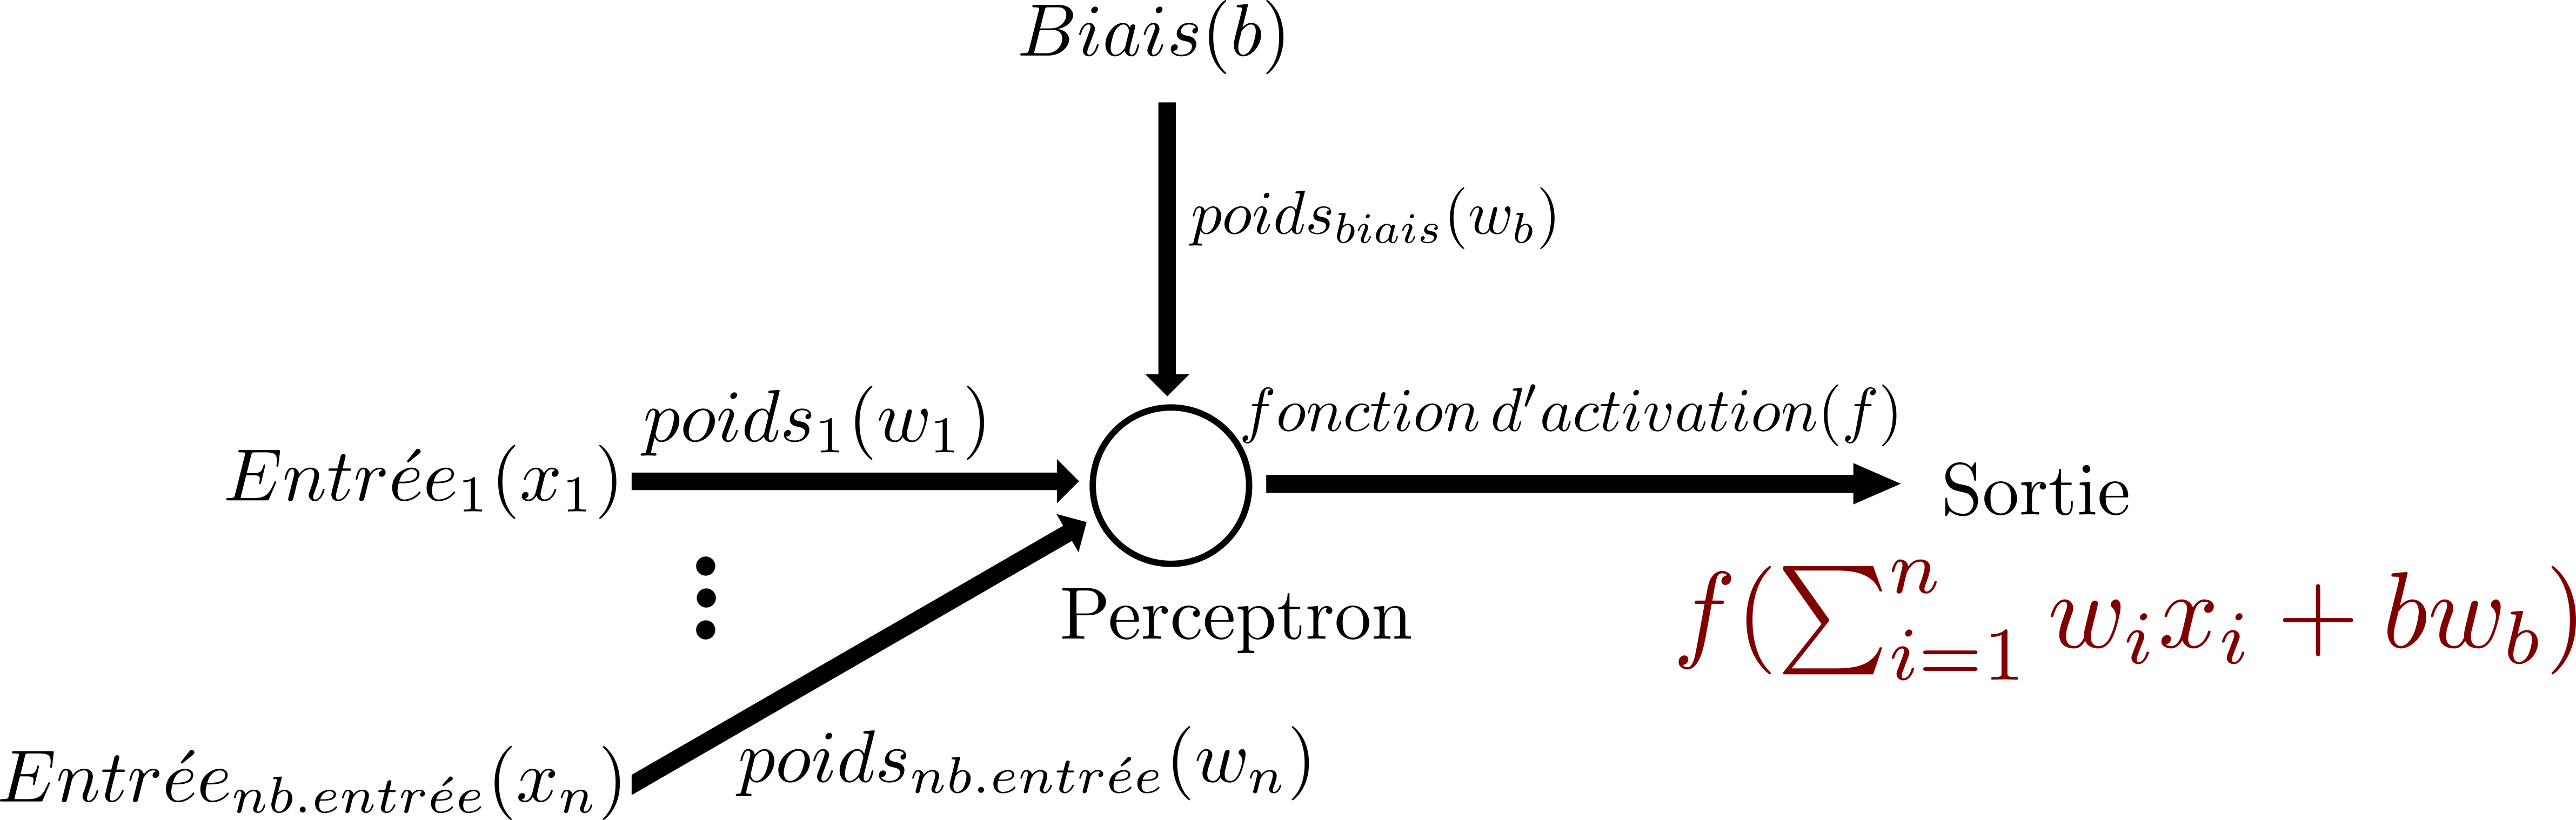
\includegraphics[height=75px]{1-Perceptron.png}
	\caption{Schéma d'un perceptron}	
\end{figure}
\begin{multicols}{2}
$
f
\left(
\begin{pmatrix}
x_1 & \ldots & x_n & b
\end{pmatrix}
\times
\begin{pmatrix}
w_1 \\
\vdots \\
w_n \\
w_b
\end{pmatrix}
\right)
$ \\
La complexité est en $O(n)$
\columnbreak
\lstinputlisting[language=Python]{code.py}
\end{multicols}
\end{frame}


\begin{frame}{II - Fonction d'activation}
\begin{figure}
	\begin{subfigure}[]{0.3\textwidth}
		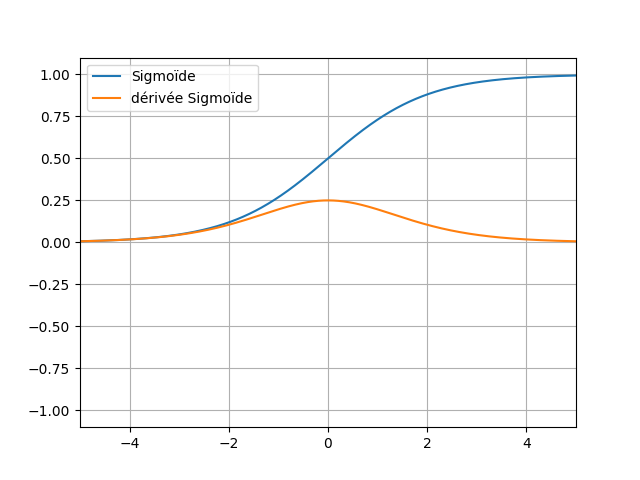
\includegraphics[width=90px]{0-Sigmoide.png}
  		\caption{Sigmoïde}
	\end{subfigure}
	\begin{subfigure}[]{0.3\textwidth}
		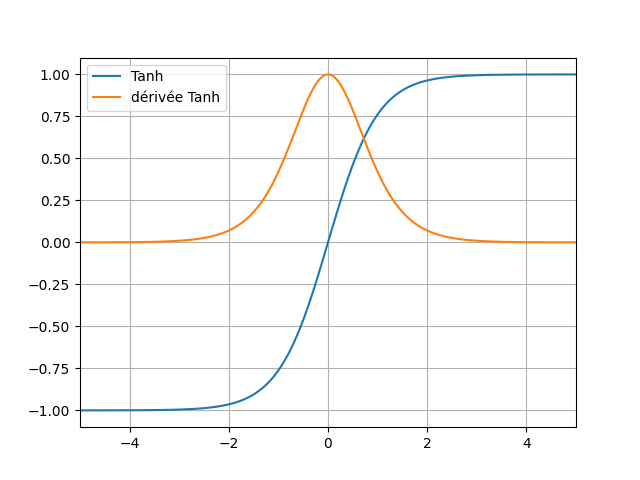
\includegraphics[width=90px]{0-Tanh.png}
  		\caption{Tanh}
	\end{subfigure}
	\begin{subfigure}[]{0.3\textwidth}
		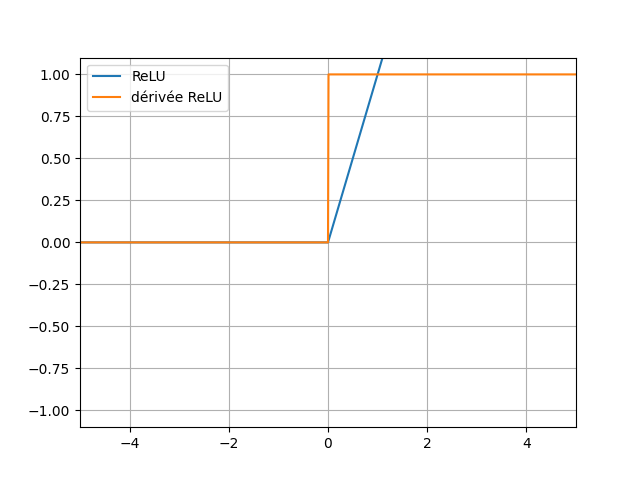
\includegraphics[width=90px]{0-ReLU.png}
		\caption{ReLU}
	\end{subfigure}
\end{figure}

\begin{block}{}
\centering
\begin{tabular}{ l || c | c | }
   Fonction & Formule & Dérivée \\ \hline \\
   Sigmoïde (a) & $\mathlarger{\frac{1}{1+e^{-x}}}$ & $f(x) \times (1-f(x))$ \\ \\
   Tangente Hyperbolique (Tanh) (b) & $\mathlarger{\frac{e^{x}-e^{-x}}{e^{x}-e^{-x}}}$ & $1-f(x)^2$ \\ \\
   Unité Linéaire Rectifiée (ReLU) (c) & $max(0, x)$ & $ \left\{\begin{array}{ll}
      														  0 & \mbox{si } x<0 \\
     														  1 & \mbox{sinon }   \end{array}\right.$ \\
\end{tabular}
\end{block}
\end{frame}

\begin{frame}{II - Fonction d'activation, les spécificités}


\begin{block}{}
\centering
\begin{tabular}{ |p{0.15\textwidth}||p{0.35\textwidth}|p{0.35\textwidth} | }
\hline 
   Fonction & Avantage & Inconvénient \\ [20pt] \hline \hline 
   Sigmoïde & A valeur dans ]0, 1[ ce qui facilite les classifications binaires & Dérivée petite vers $\pm\infty$, il y a peu d'apprentissage pour ces valeurs \\ [20pt] \hline
   Tanh & Utilisé dans les couches cachées car fonction impaire  & Même problème que la Sigmoïde \\ [20pt] \hline
   ReLU & Plus simple à calculer, prend en compte le grandient pour toute valeur positive & Dérivée nulle en x négatif ce qui peut rendre des neurones inutiles \\ [20pt] \hline 
\end{tabular}
\end{block}
\end{frame}


% 3-Descente de gradient
\section{III - Descente de gradient}
\begin{frame}{Descente de gradient}
\begin{block}{Descente de gradient}
La Descente de Gradient est un algorithme d’optimisation qui permet de trouver un minimum local d'une fonction en convergeant progressivement. \\
Dans l'apprentissage des réseaux de neurones, la descente de gradient est utilisée pour trouver le minimum d'une fonction coût, évaluant l'erreur entre la valeur de sortie du réseau et celle attendu. \\
En effet, trouver des paramètres (poids, architecture du réseau, fonction d'activation) permettant d'avoir une erreur nulle revient à résoudre le problème qu'évalue cette fonction coût par rapport aux entrées données.
\end{block}
\end{frame}

\begin{frame}{III - Descente de gradient}
\begin{block}{Algorithme du gradient}
Soit $n \in \mathbb{N}, \varepsilon > 0$. On munit $\mathbb{R}^n$ de son produit scalaire canonique. \newline
    Soit $f$ une fonction différentiable de $\mathbb{R}^n \to \mathbb{R}$. \newline
    Soit $x_0$ une valeur initiale aléatoire, $t$ le taux d'apprentissage. \newline
    Supposons $x_0, \ldots, x_k$ construits. \newline
    • Si $\norme{\nabla f(x_k)} \leq \varepsilon$, on s'arrête. \newline
    • Sinon on pose $x_{k+1} = x_k - t \nabla f(x_k)$ \newline
\end{block}

\begin{figure}
	\centering
    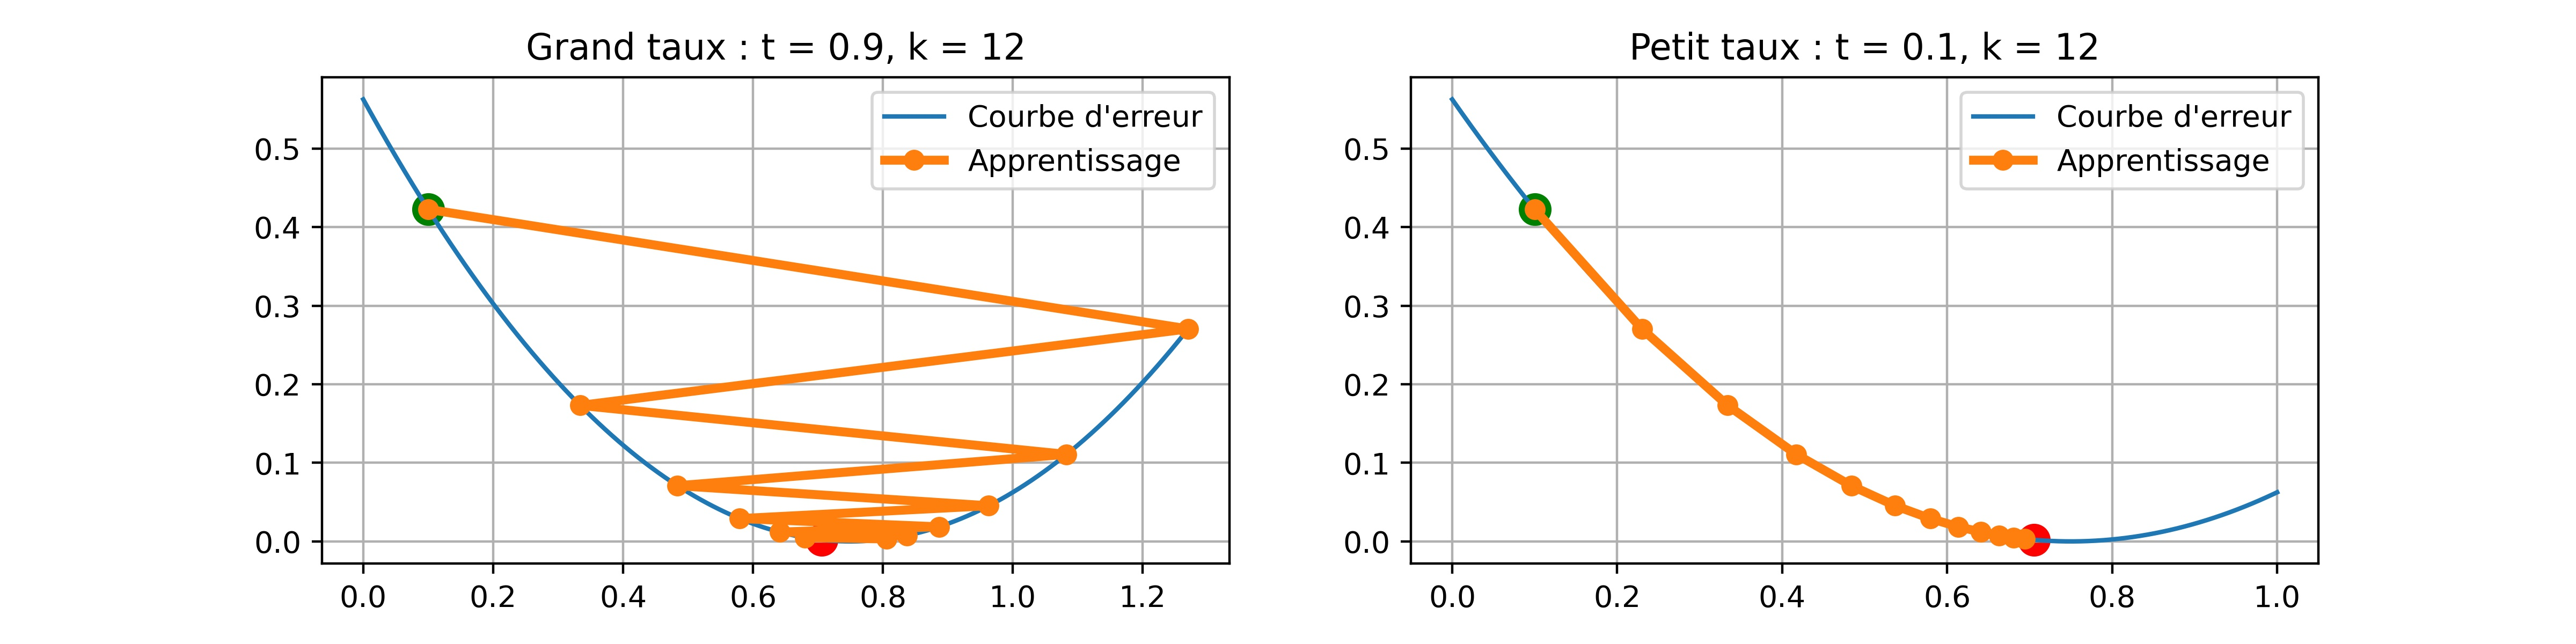
\includegraphics[height=75px]{1-DescenteGradient.jpg}
	\caption{Descente de Gradient pour $f(x) = (x-0.75)^2$; $x_0=0.1$ et $\varepsilon = 0.1$}
\end{figure}
\end{frame}

\begin{frame}{III - Importance du choix du taux d'apprentissage}
Pour la suite on continuera avec la fonction $f(x) = (x-0.75)^2$ et $x_0=0.1$. \\
On montre qu'en choisissant un taux d'apprentissage trop petit ou trop grand, il est possible que la descente de gradient diverge, ou ne converge pas assez vite.
\begin{figure}
	\centering
    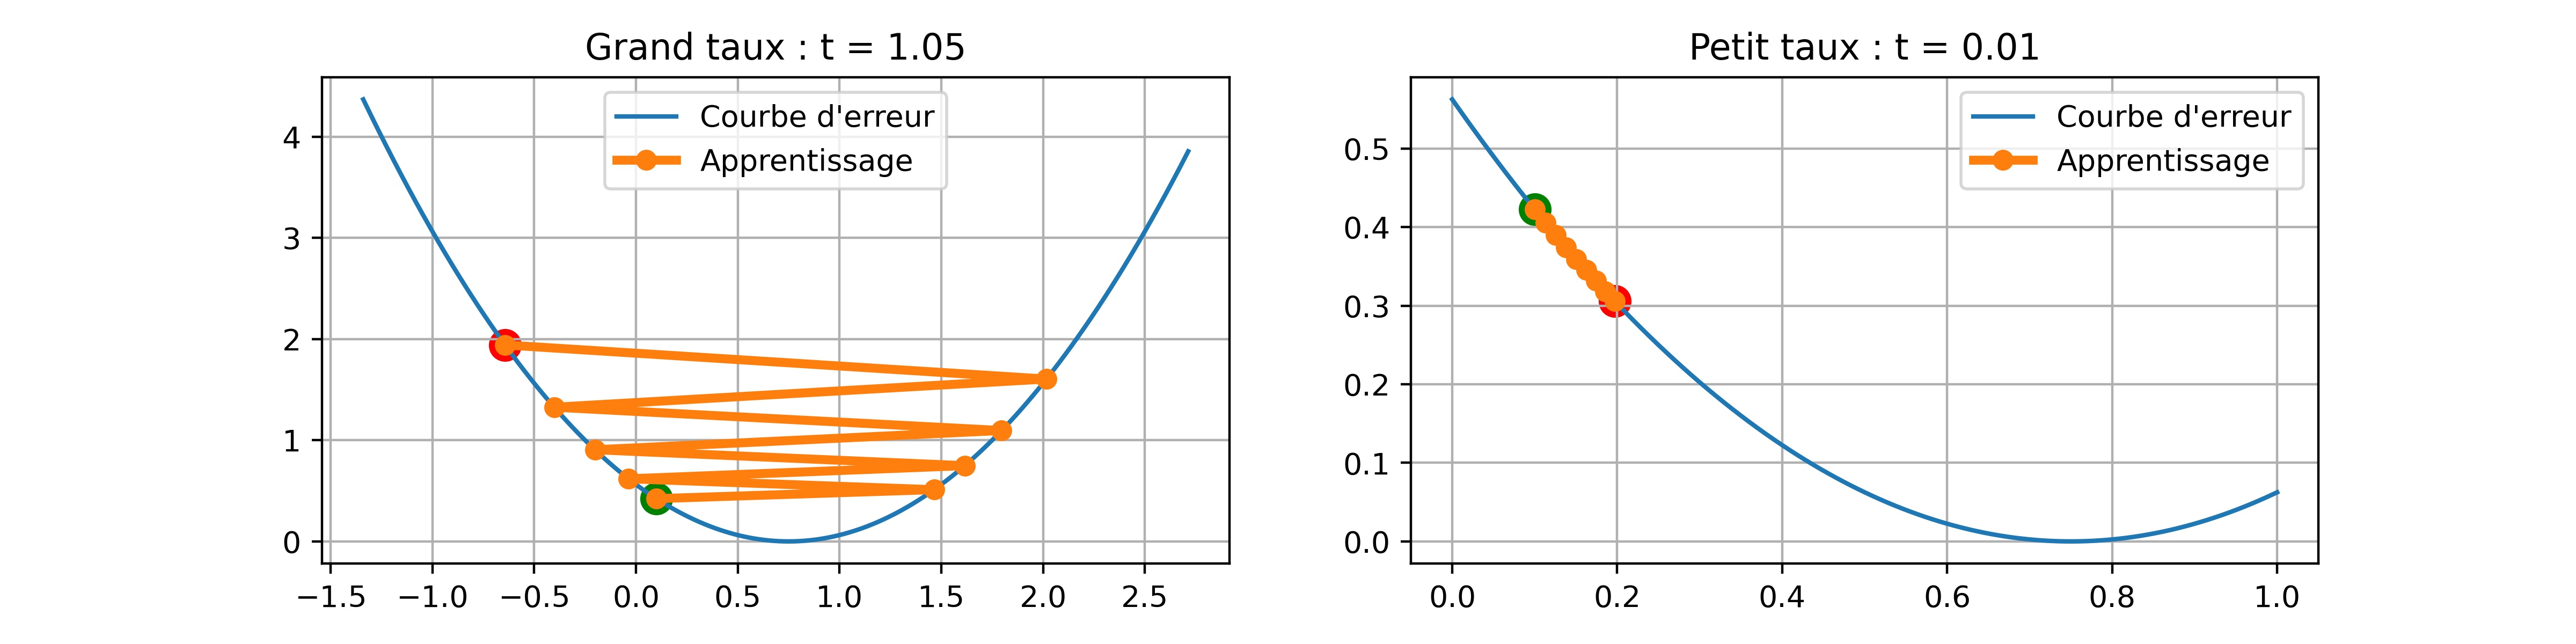
\includegraphics[height=90px]{2-DescenteGradient.jpg}
	\caption{Descente de Gradient on force l'arrêt à $k=8$}
\end{figure}
\end{frame}

\begin{frame}{III - Utilisation du Moment}
\begin{block}{Descente de gradient avec moment}
$x_0$ aléatoire et le moment $\omega_0 = 0$.
Supposons $x_0, \ldots, x_k$ et $\omega_0, \ldots, \omega_k$ construits. \\
    • On pose $\omega_{k+1} = \gamma \omega_k + t \nabla f(x_k)$ \\
    • On pose $x_{k+1} = x_k - \omega_{k+1}$ 
\end{block}
\begin{figure}
	\centering
    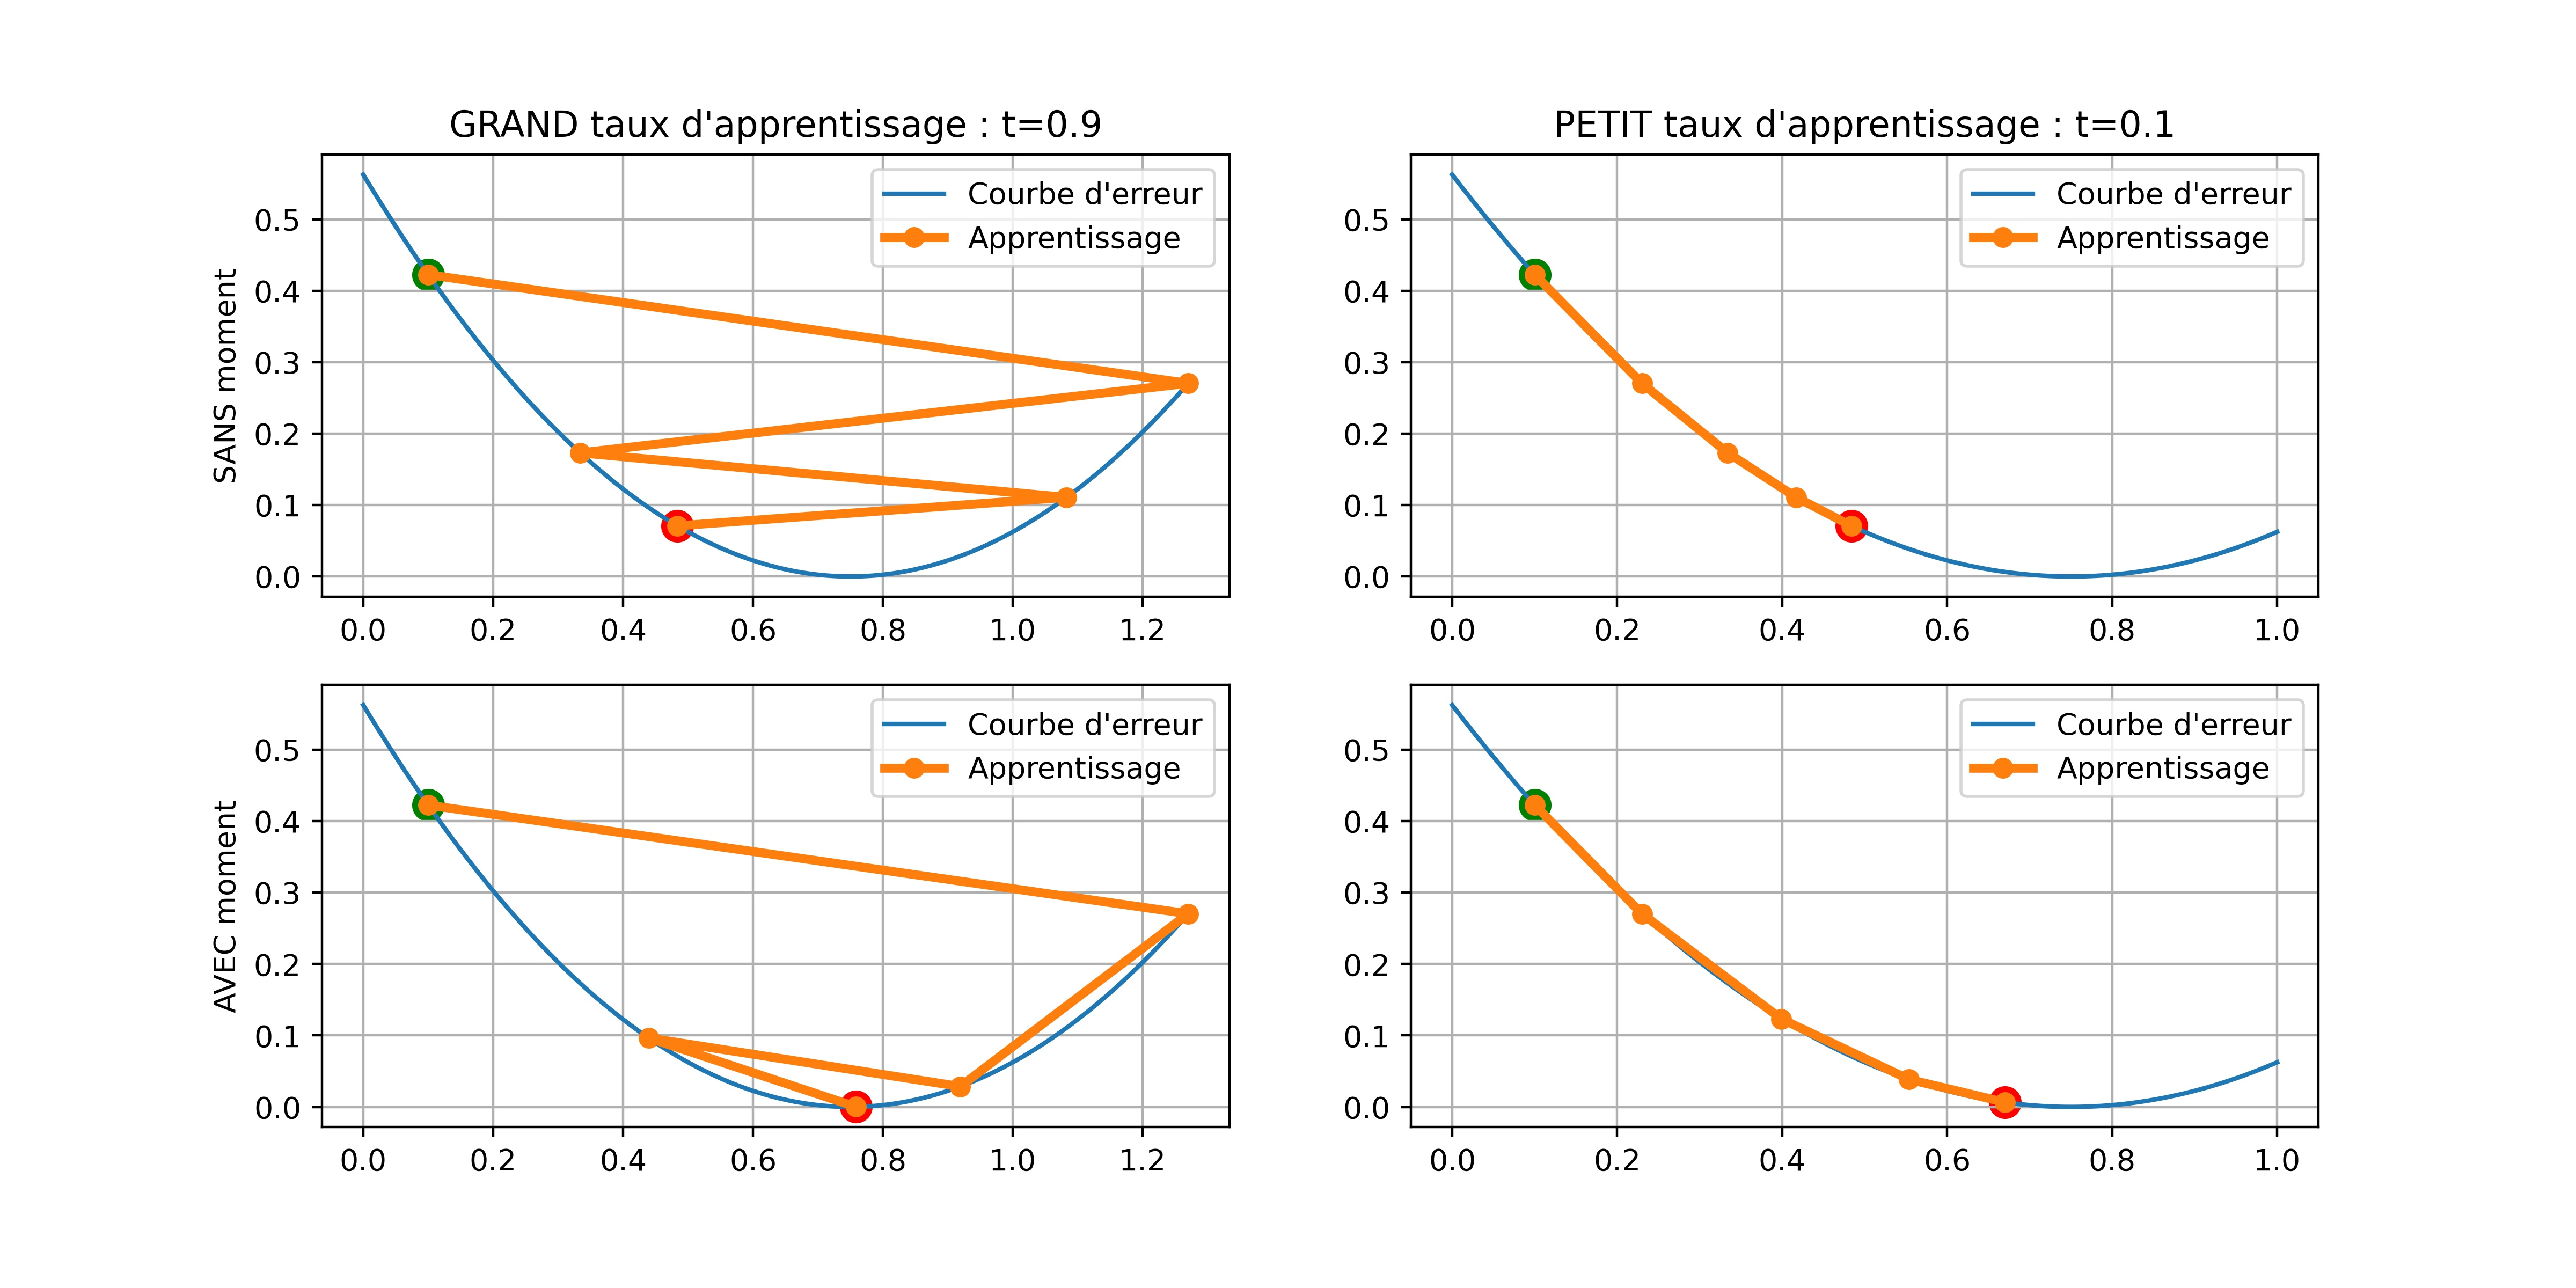
\includegraphics[height=130px, trim=0 35 0 35, clip]{3-Moment.jpg}
	\caption{Comparaison sans puis avec dépendance au moment avec $\gamma = 0.5$, arrêt à $k=4$}
\end{figure}
\end{frame}

\begin{frame}{III - Utilisation du Moment}
Le moment permet également de s'échapper de certain minimum locaux.
\begin{figure}
	\centering
    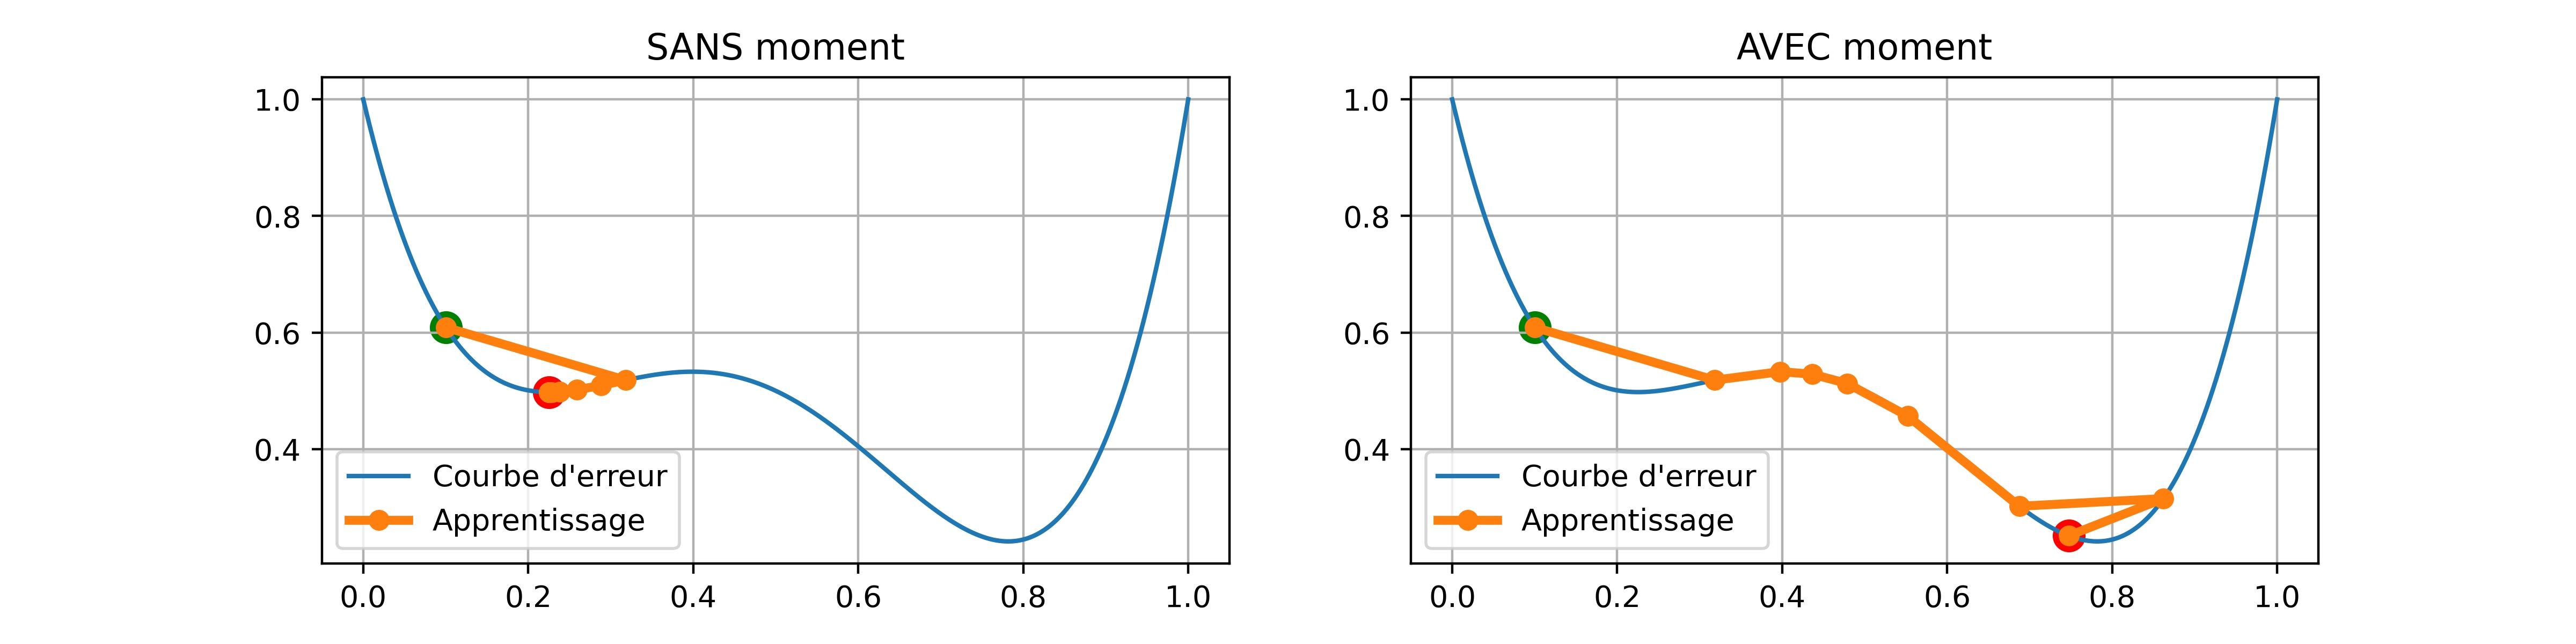
\includegraphics[width=\paperwidth, trim=0 10 0 10, clip]{4-Moment.jpg}
	\caption{Comparaison sans puis avec dépendance au moment avec $\gamma = 0.5$, arrêt à $k=8$}
\end{figure}
\end{frame}

\begin{frame}{III - Apprentissage stochastique ou par paquet (Batch)}

\begin{multicols}{2}
Il faut prendre en compte le fait que les D données d'apprentissage ne sont pas toujours juste, elles peuvent contenir des erreurs. 
\columnbreak
$
\left< f
\left(
\begin{pmatrix}
x_1^{1} & \ldots & x_n^{1} & b \\
\vdots & \vdots & \vdots & \vdots \\
x_1^{D} & \ldots & x_n^{D} & b
\end{pmatrix}
\times
\begin{pmatrix}
w_1 \\
\vdots \\
w_n \\
w_b
\end{pmatrix}
\right) \right>
$
\end{multicols}
\begin{figure}
	\centering
    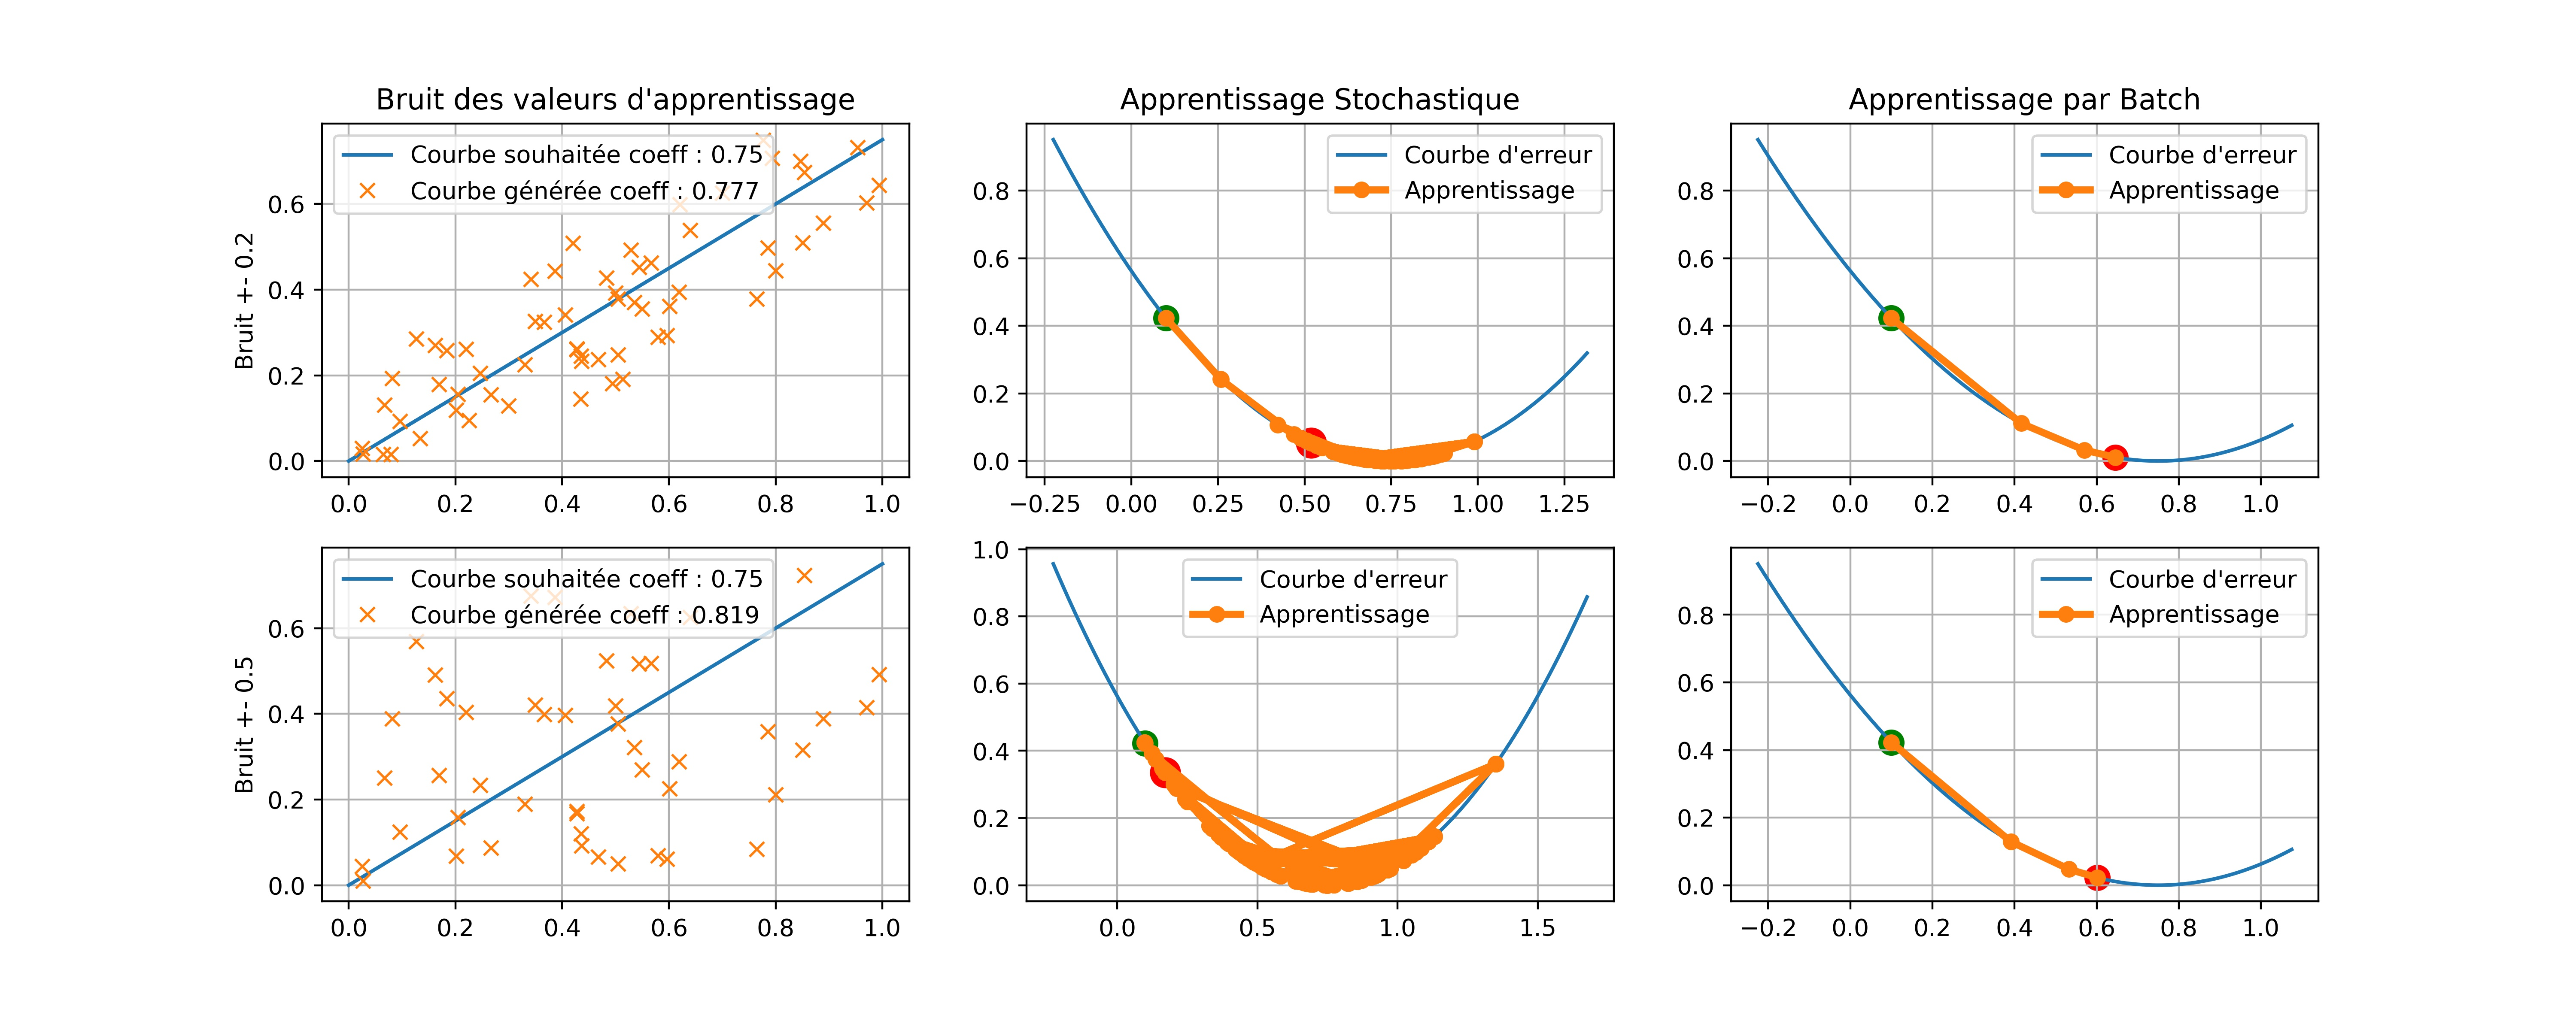
\includegraphics[width=\paperwidth, trim=0 30 0 30, clip]{5-Batch.jpg}
	\caption{Comparaison apprentissage stochastique et par paquet}
\end{figure}
\end{frame}

% 4-Problème de reproduction de l'opérateur XOR
\section{IV - Problème de reproduction de l'opérateur XOR}
\begin{frame}{IV - Problème de reproduction de l'opérateur XOR}
\begin{block}{Problème non linéairement séparables}
Un perceptron ou une couche de perceptron est incapable de reproduire des opérateurs non linéairement séparables. \\
Il faut alors mettre des couches de perceptrons en série, des couches cachées, pour reproduire ces opérateurs. \\
\end{block}
\begin{figure}
	\centering
    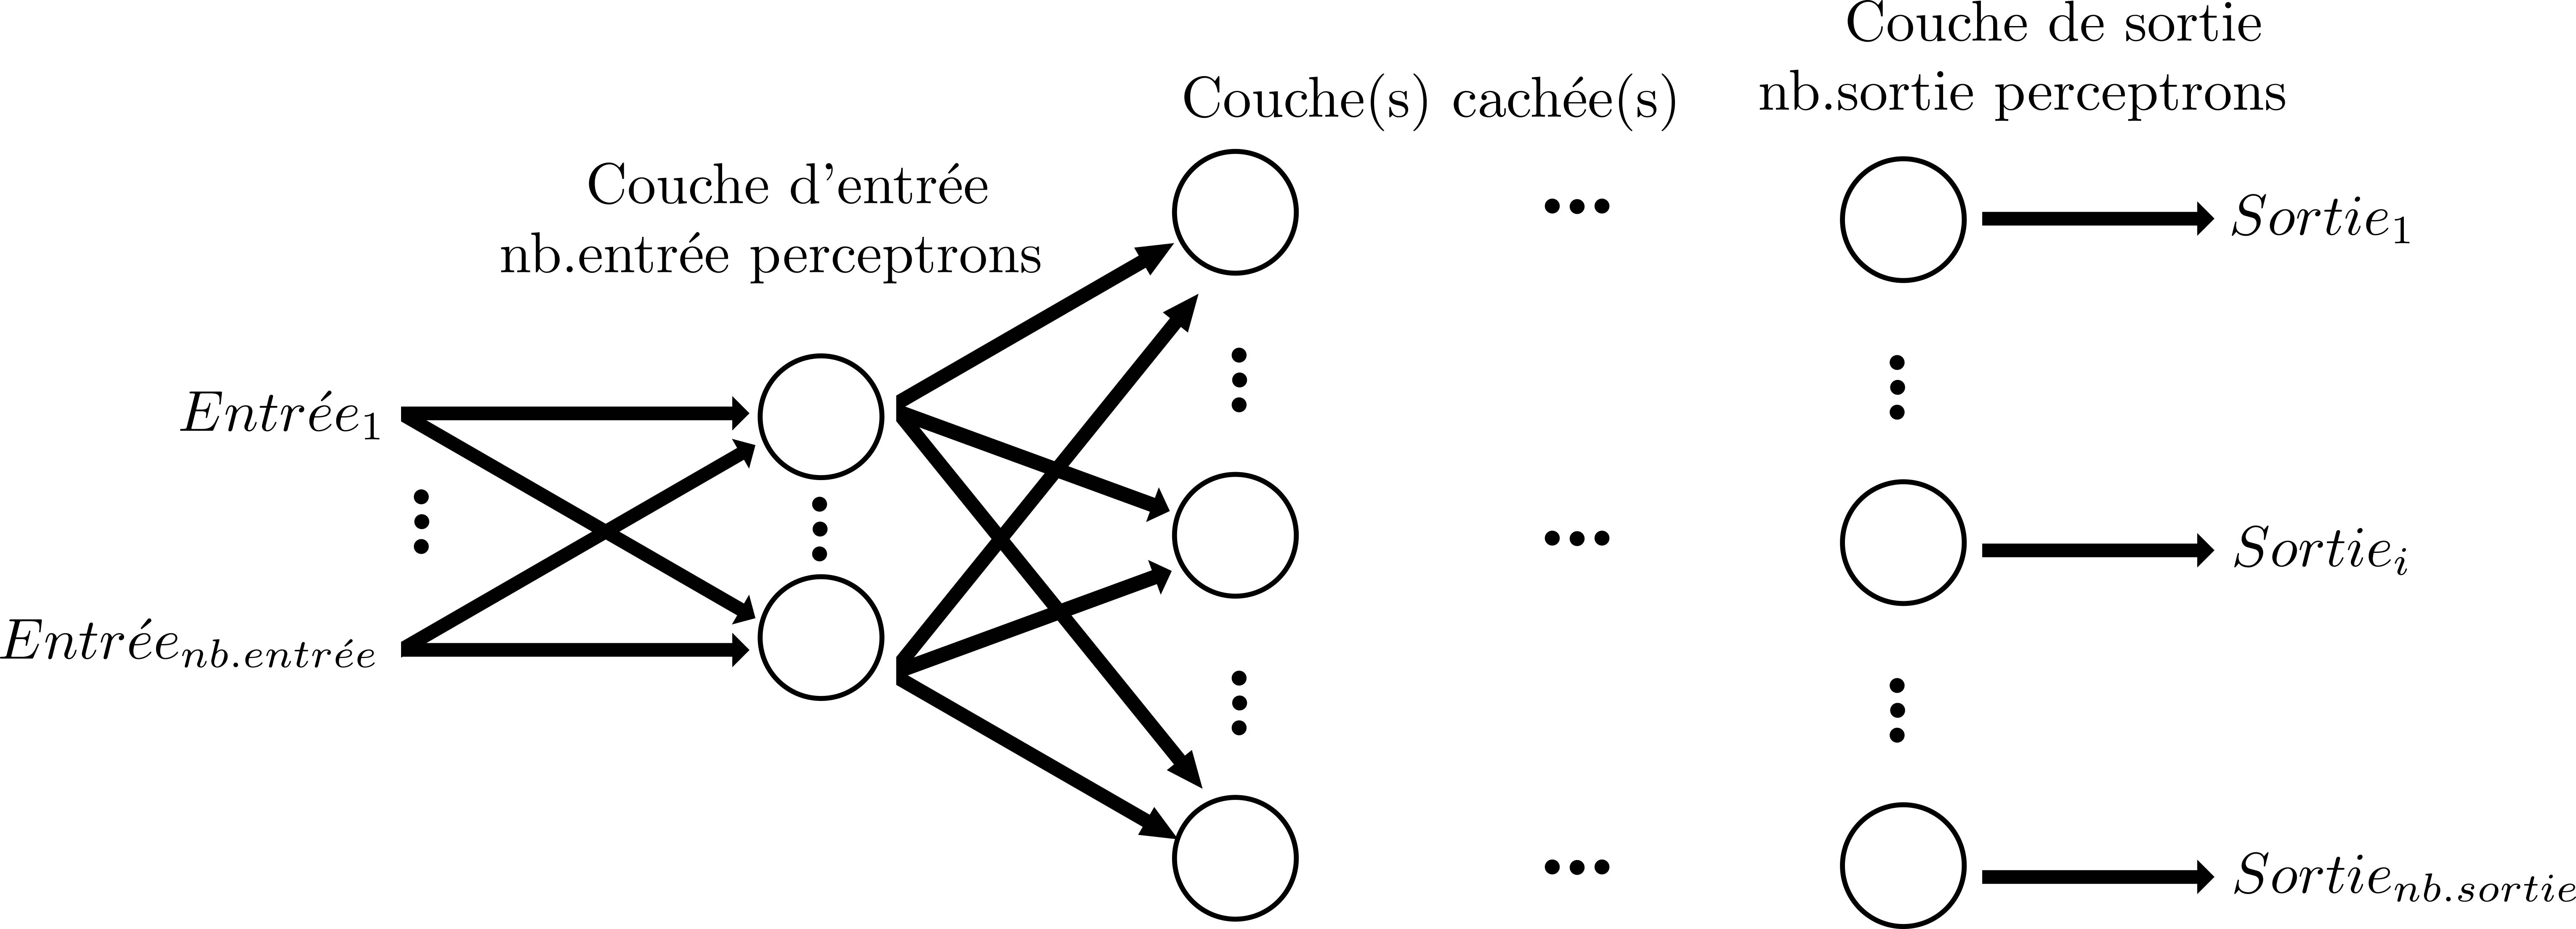
\includegraphics[width=200px]{1-Reseau.png}
	\caption{Schéma d'un réseau de neurones}
\end{figure}
\end{frame}

\begin{frame}{IV - Problème de reproduction de l'opérateur XOR}
\begin{block}{Le XOR nécessite un réseau}
Le XOR, ou exclusif, est un opérateur non linéairement séparable. \\
On peut par exemple démontrer que l'ajout d'une couche cachée de 2 perceptrons suffit à reproduire l'opérateur XOR. \\

\end{block}




\end{frame}


\end{document}